\section{\huge{Bonusopgaver}}

\subsection{Den hyggelige opgave}

Forbind prikkerne.

\begin{center}
\includegraphics[width=.99\textwidth]{forbind-prikkerne.pdf}
\end{center}


\newpage
\subsection{Rus opgaven}
Da årets rus er blevet snydt for at starte fra Scratch har vi inkluderet et
lille julepuslespil. Klip puslespillet ud sæt det sammen og udfyld, så katten
drejer én omgang.
\hspace*{-0.15\textwidth}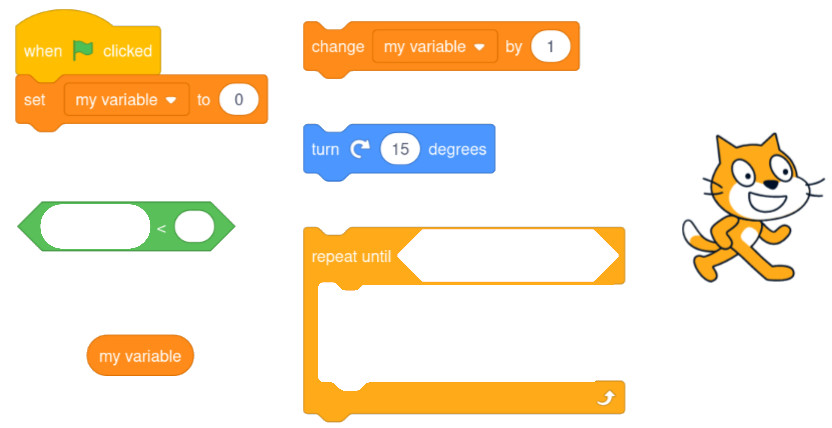
\includegraphics[width=1.3\textwidth]{figures/scratch.jpg}
\vspace{-.8cm}
\subsection{2. års rus opgaven}
\vspace*{-.1cm}
Implementer et \verb|AND| kredsløb med \verb|NAND| og \verb|INV|.\\
\vspace*{-.75cm}
\begin{center}
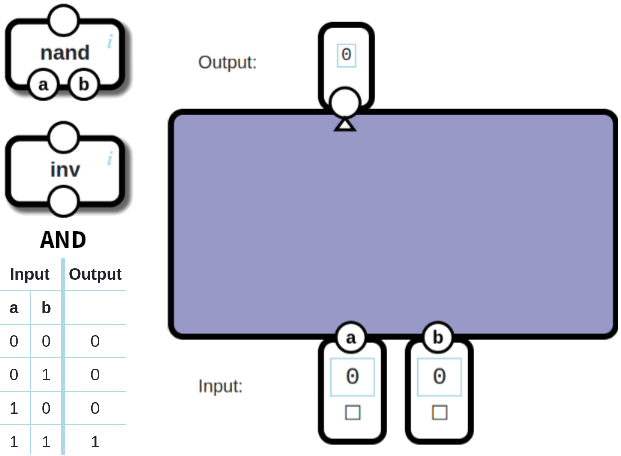
\includegraphics[width=1\textwidth]{figures/compsys.png}
\end{center}

\subsection{3. års opgaven}
Antag at du har tilvalgt LICS, men har glemt bogen. Du er kommet gennem
\verb|n|de flaske snaps og prøver nu at forklare din ven, at gud
eksisterer eller ikke eksiterer. Efter at gruble lidt har du fået følgende
skrevet ned:
\begin{align*}
    \frac{P}{P\vee Q}\vee i
    \quad\quad\frac{P\rightarrow \bot}{\neg P}\neg i
    \quad\quad\frac{P,\neg P}{\bot}\neg e
    \quad\quad\frac{\neg\neg\neg P}{\neg P}\neg\neg e
\end{align*}
Vis nu at:
\begin{align*}
   \frac{}{P \vee \neg P}
\end{align*}

\subsection{De små opgaver}
\vspace{-0.1cm}

\subsubsection{Underopgave 0}
\vspace{-0.2cm}

Donald kan godt lide primtal, men kender kun primtallene op til 2. Hjælp ham
ved at lave en F\# (eller SML) funktion, der finder alle primtal under 100.

\subsubsection{Underopgave 1}

Donald elsker IEEE standarder og har for nyligt fundet IEEE 754 til
repræsentation af tal. Hjælp ham med at omskrive tallet $173.8$ til dets
32-bit IEEE 754 repræsentation. Blev der mistet præcision?


\subsubsection{Underopgave 2}
\vspace{-0.2cm}

Implementér en x64-simulator i C.

Husk at indentere med mellemrum og ikke lave for lange linjer.

\newpage

\subsubsection{Underopgave 3}
\vspace{-0.2cm}

Håndkør følgende Whitespace-program og rapportér dets output:
\begin{verbatim}


\end{verbatim}

\subsection{C opgaven}
Omskriv følgende x86-64 assembly kode til C kode uden brug af \verb|goto|
statements
\lstdefinelanguage
   [x64]{Assembler}     % add a "x64" dialect of Assembler
   [x86masm]{Assembler} % based on the "x86masm" dialect
   % with these extra keywords:
   {morekeywords={CDQE,CQO,CMPSQ,CMPXCHG16B,JRCXZ,LODSQ,MOVSXD, %
                  POPFQ,PUSHFQ,SCASQ,STOSQ,IRETQ,RDTSCP,SWAPGS, %
                  rax,rdx,rcx,rbx,rsi,rdi,rsp,rbp, %
                  r8,r8d,r8w,r8b,r9,r9d,r9w,r9b, %
                  r10,r10d,r10w,r10b,r11,r11d,r11w,r11b, %
                  r12,r12d,r12w,r12b,r13,r13d,r13w,r13b, %
                  r14,r14d,r14w,r14b,r15,r15d,r15w,r15b}} % etc.
% Skud ud til https://tex.stackexchange.com/questions/51645/x86-64-assembler-language-dialect-for-the-listings-package
\begin{lstlisting}[language={[x64]Assembler}]
program:
    movq (%rdi), %rax
    testq %rax, %rax
    je L1
    addq $8, %rdi
    movq %rax, %rdx
L3:
    cmpq %rdx, %rax
    cmovl %rdx, %rax
    addq $8, %rdi
    movq -8(%rdi), %rdx
    testq %rdx, %rdx
    jne L3
L1:
    ret
\end{lstlisting}
[Compsys eksamen, 2017]\\
\textbf{Diskuter med en der har/ikke har haft ACS:} Føler du dig bedre
rustet til opgaven efter ACS?
\subsection{Sudoku}
\begin{center}
    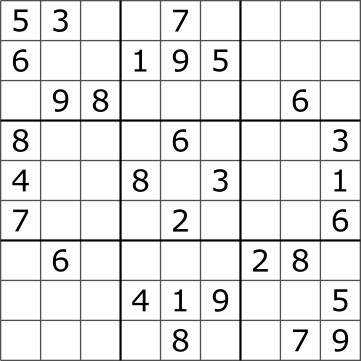
\includegraphics[width=0.4\textwidth]{figures/sudoku.jpg}
\end{center}

\newpage

\subsection{Den skægge opgave}

Santa's Quantum-Blockchain-AI-printer has broken down after he got his new
quantum bits from the Physicist. Therefore he can't use it to print the name
tags for all the presents.

Luckily an elf just found his old printer in the garage,
there's just one problem. While it can print a name tag for each child, it has
a bug that means it will print the same name for each present. He decides that
the only fair solution is to pick the name to be the one that is closest to
every child in the worlds name and use that name, then surely no one can
complain. By close he means the number of letters he needs to replace to change
one name into another. So the name Mathias and Matthew would be a distance of 4
from each other, and one name closest to both could be Mathiew, as this is only
2 replacements from each.

\begin{center}
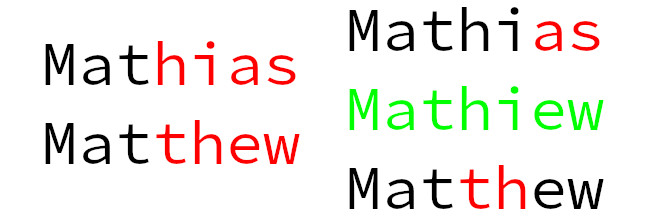
\includegraphics[width=.9\textwidth]{figures/mathias.jpg}
\end{center}

Now he just needs to figure out some way of finding
the name that's closest to the name of every child in the world before the end
of the night so he can get the printer started, and just maybe Christmas can be
saved (read: at most polynomial time).

Feel free to ask the toastmaster for the list of names, but of course they are encrypted so as to apply with GDPR

\vspace{0.5em}\textbf{\emph{NB:\@ Der udloddes en flaske snaps til den første som kommer op i
baren med en korrekt besvarelse af denne opgave!}}
